\documentclass[border=10pt]{standalone}
\usepackage{tikz}
\usetikzlibrary{automata, positioning, arrows.meta}

\begin{document}
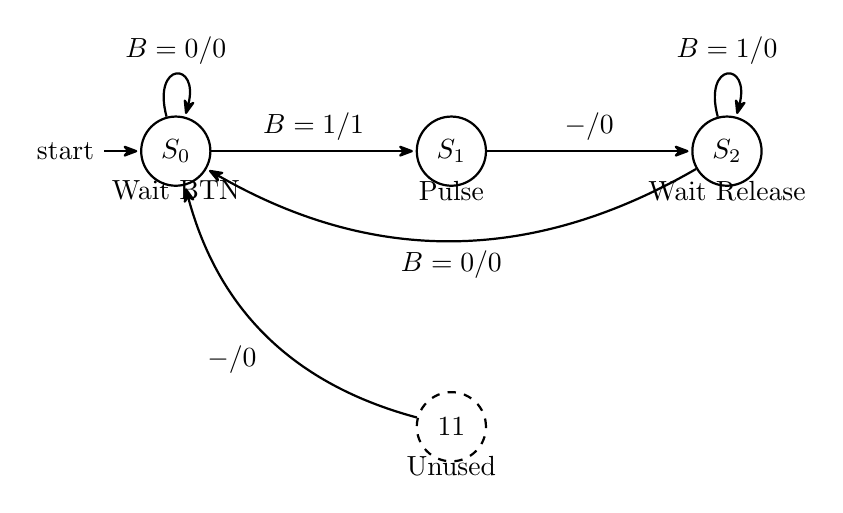
\begin{tikzpicture}[shorten >=1pt, node distance=3.5cm, on grid, auto, >={Stealth[round]}, thick]
    % States
    \node[state, initial left] (s0) {$S_0$};
    \node[state] (s1) [right=of s0] {$S_1$};
    \node[state] (s2) [right=of s1] {$S_2$};

    % Transitions
    % Mealy: Input/Output
    % S0 -> S0: B=0 / S=0
    % S0 -> S1: B=1 / S=1
    % S1 -> S2: Always (B=X) / S=0
    % S2 -> S2: B=1 / S=0
    % S2 -> S0: B=0 / S=0
    
    % Unused State
    \node[state, dashed] (s3) [below=of s1] {11};
    \node[below=0.5cm of s3] {Unused};

    \path[->]
        (s0) edge [loop above] node {$B=0/0$} (s0)
             edge node {$B=1/1$} (s1)
        (s1) edge node {$-/0$} (s2)
        (s2) edge [loop above] node {$B=1/0$} (s2)
             edge [bend left] node {$B=0/0$} (s0)
        (s3) edge [bend left] node[below left] {$-/0$} (s0);

    % Labels
    \node[below=0.5cm of s0] {Wait BTN};
    \node[below=0.5cm of s1] {Pulse};
    \node[below=0.5cm of s2] {Wait Release};

\end{tikzpicture}
\end{document}
